% Lyapunov Function Contours
% TikZ diagram for Chapter 2

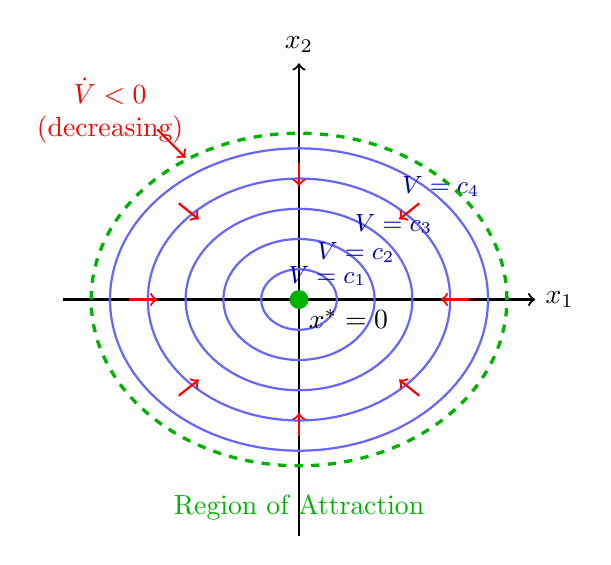
\begin{tikzpicture}[scale=1.2]
    % Axes
    \draw[->, thick] (-2.5, 0) -- (2.5, 0) node[right] {$x_1$};
    \draw[->, thick] (0, -2.5) -- (0, 2.5) node[above] {$x_2$};

    % Lyapunov function contours (ellipses for quadratic V)
    \foreach \r in {0.4, 0.8, 1.2, 1.6, 2.0} {
        \draw[blue!60, thick] (0, 0) ellipse ({\r} and {\r*0.8});
    }

    % Gradient vectors (arrows pointing inward)
    \foreach \angle in {0, 45, 90, 135, 180, 225, 270, 315} {
        \pgfmathsetmacro{\x}{1.8*cos(\angle)}
        \pgfmathsetmacro{\y}{1.8*0.8*sin(\angle)}
        \pgfmathsetmacro{\dx}{-0.3*cos(\angle)}
        \pgfmathsetmacro{\dy}{-0.3*0.8*sin(\angle)}
        \draw[->, thick, red] (\x, \y) -- +(\dx, \dy);
    }

    % Equilibrium point
    \fill[green!70!black] (0, 0) circle (0.1) node[below right, black] {$\vect{x}^* = \vect{0}$};

    % Contour labels
    \node[blue!70!black] at (1.5, 1.2) {\small $V = c_4$};
    \node[blue!70!black] at (1.0, 0.8) {\small $V = c_3$};
    \node[blue!70!black] at (0.6, 0.5) {\small $V = c_2$};
    \node[blue!70!black] at (0.3, 0.25) {\small $V = c_1$};

    % Arrows indicating decrease
    \node[red, align=center] at (-2, 2) {$\dot{V} < 0$\\(decreasing)};
    \draw[->, thick, red] (-1.5, 1.8) -- (-1.2, 1.5);

    % Region of attraction
    \draw[dashed, green!70!black, very thick] (0, 0) ellipse ({2.2} and {1.76});
    \node[green!70!black] at (0, -2.2) {Region of Attraction};

\end{tikzpicture}
